\documentclass[../main.tex]{subfiles}
\begin{document}
Chương này đồ án trình bày về các cơ sở lý thuyết toán quan trọng phục vụ cho việc xây dưng thuật toán ở chương \ref{chapter:Methodology}. Bao gồm các kiến thức về cấu trúc lý thuyết số nhóm giao hoán, nhóm nhân modulo, trường và trường hữu hạn. Trong cơ sở lý thuyết đồ án trình bày hệ mật đường cong Elliptic - hệ mật được dùng trong thử nghiệm thực tế trong chương \ref{chapter:Experiment}.

\section{Lý thuyết số tính toán}
\subsection{Nhóm cyclic}
\label{section: theory_background}
\begin{dn}
Một nhóm $X$ được gọi là \textbf{cyclic} nếu $X$ có hệ sinh là một phần tử: $\{g\} \subset X$. Phần tử $g$ khi đó được gọi là phần tử sinh của $X$.
\end{dn}
\begin{nx}
Giả sử $(G,\cdot)$ là một nhóm với phần tử đơn vị $e$ và $g \in G$. Ta xét nhóm con cyclic sinh bởi $g$. Có hai trường hợp xảy ra như sau:
\begin{enumerate}
    \item Nếu $g^\alpha \neq g^\beta$ với mọi $\alpha \neq \beta$ thì nhóm cyclic $\langle g \rangle = \{g^k \mid k \in \mathbb{Z}\}$
    \item Nếu tồn tại hai số nguyên $\alpha \neq \beta$ sao cho $g^\alpha = g^\beta$ thì vì $g^{\alpha - \beta} = g^{\beta - \alpha} = e$ nên luôn tồn tại số nguyên dương $m$ để $g^m = e$. Gọi $n$ là số nguyên dương nhỏ nhất sao cho $g^n = e$. Khi đó 
    $$\langle g \rangle = \{e,g,g^2,...,g^{n-1}\} $$
    có cấp là $n$ và $g^k = e$ khi và chỉ khi $k$ chia hết cho $n$.
\end{enumerate}
\end{nx}


\begin{dn}
\subsection{Nhóm nhân Modulo}
Nhóm nhân modulo $p$, ký hiệu là $\mathbb{Z}^*_p$. Là một tập gồm $\phi(p)$ phần tử. Với $p$ là số nguyên tố thì $\mathbb{Z}^*_p$ gồm $p-1$ phần tử ${1,2,...,p-1}$ dưới toán tử nhóm nhân modulo $p$. 
\end{dn}
\begin{nx}
$\mathbb{Z}^*_p$ thỏa mãn các tính chất của nhóm Abel:
\begin{enumerate}
    \item Hai phần tử bất kì trong tập nhân với nhau modulo $p$ thì cho kết quả thuộc tập hợp.
    \item Phần tử 1 là phần tử đơn vị, tức là $1\cdot x = x = x \cdot 1$ với mọi phần tử $x$ trong tập hợp.
    \item Mọi phần tử $x$ đều tồn tại phần tử nghịch đảo $x^{-1}$ sao cho $xx^{-1} = 1 = x^{-1}x$ (mod $p$).
    \item Với mọi phần tử $a,b,c$ trong tập, $a(bc) = (ab)c$ (mod $p$).
    \item Với hai phần tử $a,b$ trong tập, $ab = ba$ (mod $p$).
\end{enumerate}

\end{nx}

Tính chất 4 và 5 là kế thừa từ tính chất của phép nhân trong $\mathbb{Z}$ và cũng như phần tử đơn vị trong tính chất 2. Để chỉ ra tính chất 1 đúng, ta cần chỉ ra tích của hai phần tử trong tập hợp không bao giờ bằng không. Giả sử $xy \equiv 0$$\pmod p$ với $x,y$ trong tập hợp. Điều này ngụ ý rằng hoặc $x$ hoặc $y$ chia hết cho $p$. Điều này dẫn tới mâu thuẫn.

Để chứng minh rằng mọi phần tử đều tồn tại phần tử nghịch đảo. Ta để ý rằng $\gcd(x,p) = 1$. Điều này có nghĩa tồn tại hai số nguyên $r$, $s$ sao cho $xr + ps =1$. Ta có thể viết lại $xr = 1 - px$ hay $xr \equiv 1 \pmod p$. Ta kết luận rằng $r$ (hoặc $r\pmod p$) là nghịch đảo của $x$.

Với phần tử $a \in (G,*)$  xác định $a^n$ bởi $a = a*a*\dots*a$ [$n$ lần]. Với nhóm $\mathbb{Z}^*_p$ ký hiệu $a^n$ tương ứng với phép toán mũ modulo, ở đó $a^n$ là phần tử thu được từ phần tử $a$ và nhân với bản thân nó $n$ lần$\mod p$.
Từ đó ta có thể xác định luật mũ.
\begin{enumerate}
    \item $a^mb^m = (ab)^m$
    \item $a^ma^n = a^{m+n}$
    \item $(a^m)^n = a^{mn}$
\end{enumerate}

Để ý rằng $m,n$ là các số nguyên không phải các phần tử của nhóm. Do đó ta có thể thực hiện phép toán cộng và phép toán nhân một cách bình thường. Với số mũ bằng không, $a^0 =1$.

\begin{dl}
(Định lý Fermat nhỏ) Với mọi phần tử $a \in \mathbb{Z}^*_p$ ta có $a^{p-1} = 1$. 
\end{dl}

Để tìm phần tử sinh của nhóm cyclic $\mathbb{Z}^*_p$ ta có hai cách và cả hai đều có thể triển khai số nguyên tố lớn $p$. 

Cách thứ nhất là chọn một phần tử $a \in \mathbb{Z}^*_p$ và chỉ ra rằng $a^i \neq 1$ với mọi $i = 1,2,...,p-2$. Điều này dẫn đến số lượng phép tính lớn khi $p$ lớn.

Cách thứ hai là phân tách $p-1$ và sử dụng tính chất rằng $a$ là phần tử sinh khi và chỉ khi $a^{(p-1)/q} \not\equiv 1\pmod  p$ với mọi số nguyên tố $q$ là ước của $p-1$. Vì thế ta cần thử ứng viên đối với các ước nguyên tố của $p-1$. Nhưng tuy vậy bài toán phân tích thừa số nguyên tố cũng là một bài toán khó.

\begin{vd} Phần tử sinh với $p = 11$
\end{vd}

Với số nguyên tố $p =11$, ta có $\mathbb{Z}^*_{11} = \{1,2,...,10\}$ với bậc $10 = p-1$.
Xét phần tử sinh $g = 2$ và các phần tử được sinh bởi nó (các tính toán đều được lấy modulo $p$).
$$ \langle 2 \rangle = \{ 2,4,8,5,10,9,7,3,6,1\} = \mathbb{Z}^*_{11}
$$

Với phần tử sinh $g = 3$ chỉ sinh ra nhóm con có bậc bằng 5.
$$ \langle 3 \rangle = \{3,9,5,4,1\} 
$$

Và phần tử sinh $g = 10$ chỉ sinh ra nhóm con có hai phần tử.
$$ \langle 10 \rangle = \{10,1\} 
$$

Ta có thể tính toán tất cả các nhóm con được sinh ra từ mỗi phần tử trong $\mathbb{Z}^*_{11}$ như trong bảng \ref{fig:subCyclic}.

\begin{table}[h!]
    \centering
    
    \begin{tabular}{||c c c||}
    \hline
    $g$  & $\langle g \rangle$        & Bậc($\langle g \rangle$)   \\
    \hline \hline
    1  & \{1\}                    & 1  \\
    2  & \{2,4,8,5,10,9,7,6,1\}   & 10 \\
    3  & \{3,9,5,4,1\}            & 5  \\
    4  & \{4,5,9,3,1\}            & 5  \\
    5  & \{5,3,4,9,1\}            & 5  \\
    6  & \{6,3,7,9,10,5,8,4,2,1\} & 10 \\
    7  & \{7,5,2,3,10,4,6,9,8,1\} & 10 \\
    8  & \{8,9,6,4,10,3,2,5,7,1\} & 10 \\
    9  & \{9,4,3,5,1\}            & 5  \\
    10 & \{10,1\}                 & 2 \\
    \hline
    \end{tabular}
    \caption{Bảng các nhóm con cyclic của $\mathbb{Z}_{11}^*$}
    \label{fig:subCyclic}
\end{table}
\begin{nx}
Với bất kỳ một số nguyên tố $p$ ta đều có
\begin{enumerate}
    \item Nhóm con sinh bởi phần tử 1 luôn luôn có bậc là một.
    \item Nhóm con sinh bởi phần tử $p-1$ có bậc là 2, do $(p-1)^2 =p^2 -2p +1 \equiv 1\pmod p$.
    \item Có đúng $\phi(p-1)$ phần tử sinh ra toàn bộ nhóm, trong đó $\phi(n)$ là hàm phi Euler, số các số nguyên dương nhỏ hơn $n$ và nguyên tố cùng nhau với $n$.
\end{enumerate}
\end{nx}

Trong ví dụ $p = 11$. Ta có đúng $\phi(11-1)$ phần tử sinh ra toàn bộ nhóm $\mathbb{Z}^*_{11}$. Cụ thể là $\langle 2 \rangle = \langle 6 \rangle = \langle 7 \rangle = \langle 8 \rangle = \mathbb{Z}^*_{11}$.

Hơn nữa, nếu $d$ là ước của $p-1$ thì ta có $\phi(d)$ phần tử sinh ra nhóm con có bậc là $d$.

\subsection{Trường và trường hữu hạn}
\begin{dn}
(Trường) Trường $F$ là một tập các phần tử được trang bị hai phép toán $(+),(\cdot)$ với các tính chất sau
\begin{enumerate}

    \item $(F,+)$ tạo thành một nhóm Abel với phần tử trung hòa là 0.
    \item $(F/\{0\},\cdot)$ tạo thành một nhóm Abel với phần tử trung hòa là 1.
    \item Phép nhân trong $F$ phân phối với phép cộng trong $F$
    $$z(x+y)=zx+zy$$
    với mọi $x,y,z \in F$.
\end{enumerate}
\end{dn}
\begin{vd}
\end{vd}
\begin{itemize}
    \item Trường số thực $\mathbb{R}$ là một trường có phần tử trung hòa 0 với phép toán cộng và phần tử trung hòa 1 với phép toán nhân. Mọi số thực $a$ đều có phần tử nghịch đảo phép cộng là $-a$, mọi phần tử khác không $b$ có phần tử nghịch đảo phép nhân là $1/b$.
    \item Tập $\mathbb{Z}_p$ với hai toán tử cộng và nhân modulo $p$ là một trường. Trường này là trường hữu hạn các phần tử.
\end{itemize}

Số các phần tử của trường được gọi là bậc hoặc lực lượng của trường.
\begin{dl}
Một trường bậc $n$ chỉ tồn tại nếu n là lũy thừa của một số nguyên tố, i.e $n = p^m$ với số nguyên dương $m$ và số nguyên tố $p$. Số $p$ được gọi là đặc số của trường.
\end{dl}

\begin{vd}
\end{vd}
\begin{itemize}
    \item Trường hữu hạn có 11 phần tử $GF(11)$.
    \item Trường hữu hạn có 256 phẩn tử $GF(2^8)$.  
\end{itemize}

Các phần tử của $GF(p^m)$ là các đa thức bậc nhỏ hơn $n$ với hệ số trong $GF(p)$.
$$a_{m-1}x^{m-1} + \dots a_1x + a_0 = A(x) \in GF(p^m)
$$
Trong đó $a_i \in \mathbb{Z}_p$


Phép toán cộng và trừ trên $GF(p^m)$ được thực hiện trên các hệ số của đa thức theo $GF(p)$.
Phép toán nhân hai phần tử là phần dư của phép chia Euclidean bởi đa thức bất khả quy $P$ bậc $m$ với tích hai đa thức.

\begin{vd}
\end{vd}

Các phần tử của trường $GF(2^3)$ là các đa thức có dạng
$$ A(x) = a_2x^2 +a_1x +a_0
$$

$GF(8)$ có 8 phần tử
$$GF(2^3) = \{0,1,x,x+1,x^2,x^2+1,x^2+x,x^2+x+1\}
$$
$$A(x) = X^2+x+1
$$
$$B(x) = X^2 +1
$$
$$A(x) + B(x) = x
$$

Đa thức  bất khả quy bậc 3 $P(x) = x^3+x+1$ 
$$A(x)\cdot B(x) = x^2+x \mod P(x)
$$

Phần tử nghịch đảo $A^{-1}(x)$ của phần tử khác 0 $A(x) \in GF(2^m)$ được xác định bởi
$$A(x)\cdot A^{-1}(x) = 1 \mod P(x)
$$

\section{Đường cong Elliptic}
\subsection{Đường cong Elliptic trên trường số thực}
\begin{dn} \rm
Cho $a,b\in \mathbb{R}$ là các hằng số thỏa mãn $4a^3+27b^2\ne 0$. Một đường cong Elliptic không suy biến trên trường số thực là tập $E$ các nghiệm $(x,y)\in \mathbb{R}\times\mathbb{R}$ của phương trình Weistrass
$$y^2=x^3+ax+b,$$
cùng với một điểm đặc biệt $\mathcal{O}$ được gọi là điểm ở vô cùng.
\end{dn}
\begin{cy}
Có thể chứng minh được rằng điều kiện $4a^3+27b^2\ne 0$ là cần và đủ để đảm bảo phương trình $x^3+ax+b=0$ có 3 nghiệm phân biệt (thực và phức). Nếu $4a^3+27b^2=0$ thì đường cong Elliptic được gọi là đường cong Elliptic suy biến. Trong phạm vi đồ án này, chỉ xét các đường cong không suy biến.
\end{cy}

Để các điểm trên đường cong Elliptic tạo thành nhóm Abel, tạo ra một điểm đặc biệt, gọi là điểm ở vô cùng thêm vào đường cong, kí hiệu $\mathcal{O}$. Điểm này không tồn tại trên mặt phẳng $xy$, nhưng ta giả sử nó nằm ở trên cùng và dưới cùng của trục $y$.  Đặt $P+P'=\mathcal{O}$ thì $\mathcal{O}$ là phần tử đơn vị đối với phép cộng $P+\mathcal{O}=\mathcal{O}+P=P$ với mọi $P,P'\in E$.
\begin{dl}
\label{thm: 1}
(Thuật toán cộng trên đường cong Elliptic) Cho 
$$E\colon y^2=x^3+ax+b$$
là đường cong Elliptic và xét các điểm $P_1$ và $P_2$ trên $E$.
\begin{itemize}
\item Nếu $P_1=\mathcal{O}$ thì $P_1+P_2=P_2$.
\item Trái lại, nếu  $P_2=\mathcal{O}$ thì $P_1+P_2=P_1$.
\item Trái lại, viết $P_1=(x_1,y_1)$ và $P_2=(x_2,y_2)$.
\item Nếu $x_1=x_2$ và $y_1=-y_2$, thì $P_1+P_2=\mathcal{O}$.
\item Trái lại, định nghĩa $\lambda$ bởi:
$$\lambda=\begin{cases}
\dfrac{y_2-y_1}{x_2-x_1}&\text{nếu }P_1\ne P_2,\\
\dfrac{3x_1^2+A}{2y_1}&\text{nếu }P_1=P_2,
\end{cases}$$
và đặt
$$x_3=\lambda^2-x_1-x_2\quad \text{và}\quad y_3=\lambda(x_1-x_3)-y_1.$$
thì $P_1+P_2=(x_3,y_3)$.
\end{itemize}
\end{dl}

Phép nhân 2 điểm trên đường cong $E$ không được định nghĩa, có nghĩa là không tồn tại $P_1\times P_2$ với $P_1,P_2\in E$.

Không tồn tại thuật toán chia một điểm cho một số nguyên dương $P_2: n$. Bài toán tìm số $n$ thỏa mãn $P_2=nP_1$ là bài toán chưa có thuật toán giải trong thơi gian đa thức.
\begin{dl}
\label{thm: 2}
Cho $E$ là một đường cong Elliptic. Khi đó luật cộng trên $E$ có các tính chất sau:
\begin{enumerate}
\item Phần tử đơn vị: $P+\mathcal{O}=\mathcal{O}+P=P$ với mọi $P\in E$.
\item Phần tử nghịch đảo: $P+(-P)=\mathcal{O}$ với mọi $P\in E$.
\item Tính kết hợp: $(P+Q)+R=P+(Q+R)$ với mọi $P,Q,R\in E$.
\item Tính giao hoán: $P+Q=Q+P$ với mọi $P,Q\in E$.
\end{enumerate}
Nói cách khác, luật cộng làm cho các điểm của $E$ tạo thành một nhóm Abel.
\end{dl}

\subsection{Đường cong Elliptic trên trên $ \mathbb{Z}_p$}
Với $p>3$ là số nguyên tố. Các đường cong Elliptic trên $\mathbb{Z}_p$ được định nghĩa giống như trên trường số thực, thay các phép toán trên $\mathbb{R}$ bởi các phép toán tương ứng trên $\mathbb{Z}_p$.
\begin{dn} \rm
Cho $p>3$ là số nguyên tố. Đường cong Elliptic $y^2=x^3+ax+b$ trên trường $\mathbb{Z}_p$ là tập nghiệm $(x,y)\in\mathbb{Z}_p\times \mathbb{Z}_p$ của phép đồng dư
$$y^2\equiv x^3+ax+b\mod p,$$
ở đó $a,b\in \mathbb{Z}_p$ là các hằng số thỏa mãn $4a^3+27b^2\not\equiv 0 \mod p$, cùng với một điểm đặc biệt $\mathcal{O}$ được gọi là điểm ở vô cùng. 
\end{dn} 

Phép toán cộng trên $E$ được định nghĩa như sau: Giả sử $P_1=(x_1,y_1)$ và $P_2=(x_2,y_2)$ là các điểm trên $E$. Nếu $x_2=x_1$ và $y_2=-y_1$ thì $P_1+P_2=\mathcal{O}$; ngược lại $P_1+P_2=(x_3,y_3)$, ở đó
$$x_3=\lambda^2-x_1-x_2\quad \text{và}\quad y_3=\lambda(x_1-x_3)-y_1,$$
với
$$\lambda=\begin{cases}
\dfrac{y_2-y_1}{x_2-x_1}&\text{nếu }P_1\ne P_2,\\
\dfrac{3x_1^2+A}{2y_1}&\text{nếu }P_1=P_2.
\end{cases}$$

Cuối cùng, định nghĩa $P+\mathcal{O}=\mathcal{O}+P=P,$ với mọi $P\in E$.
\begin{cy}
Luật cộng các điểm trên đường cong Elliptic $E$ trên $\mathbb{Z}_p$ cũng xác định một nhóm Abel $(E, +)$.
\end{cy}
\subsection{Đường cong Elliptic trên trường hữu hạn}
Định nghĩa một đường cong Elliptic trên $F_q$ bởi phương trình có dạng: $E\colon y^2=x^2+ax+b,$ với $a,b\in {F}_q$ thỏa mãn $4a^3+27b^2\ne 0$ và  xét các điểm trên $E$ với các tọa độ trong $F_q$, kí hiệu
$$E({F}_q)=\left\{(x,y):x,y\in {F}_q \text{ thỏa mãn } y^2=x^2+ax+b\right\}\cup \{\mathcal{O}\}.$$
\vspace{-1cm}
\begin{dl}
Cho $E$ là  một đường cong Elliptic trên $F_q$ và lấy $P$ và $Q$ là các điểm trong $E(F_q)$.
\begin{enumerate}
\item Thuật toán cộng trên đường cong Elliptic áp dụng với hai điểm $P$ và $Q$ tạo ra một điểm trong $E(F_q)$. Kí hiệu điểm này là $P+Q$.
\item Luật cộng trên $E(F_q)$ thỏa mãn các tính chất trong nhóm giao hoán.
Hình \ref{fig:F11} biểu diễn các điểm của một đường cong Elliptic trên trường hữu hạn $F_{11}$. 

\begin{figure}[h!]
    \centering
    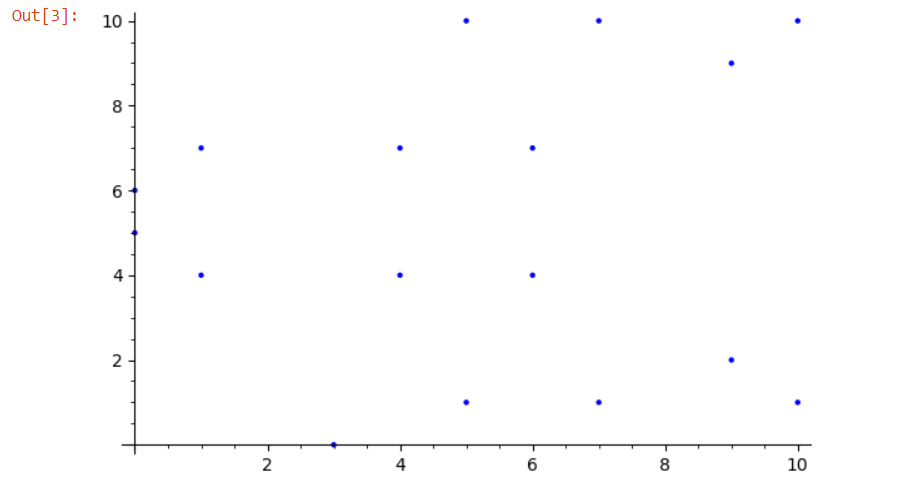
\includegraphics[scale = 0.7]{Figure/Fp.png}
    \caption{Đường cong Elliptic trên trường hữu hạn $F_{11}$}
    \label{fig:F11}
\end{figure}
\end{enumerate}
\end{dl}



\end{document}